% Build: uv run src/build_report.py   (regenerates numbers.tex from the data, then runs pdflatex)
\documentclass[11pt]{article}
\usepackage[a4paper,margin=2.3cm]{geometry}
\usepackage[T1]{fontenc}
\usepackage{lmodern,textcomp}
\usepackage{graphicx,amsmath,amssymb,booktabs,caption,microtype}
\usepackage{titlesec}
\usepackage[hidelinks]{hyperref}
\graphicspath{{../figures/}}
\captionsetup{font=small,labelfont=bf,skip=3pt}
\setlength{\parskip}{0.4em}
\setlength{\parindent}{0pt}
\setlength{\abovedisplayskip}{4pt}\setlength{\belowdisplayskip}{4pt}
\setlength{\abovedisplayshortskip}{3pt}\setlength{\belowdisplayshortskip}{3pt}
\titleformat{\section}{\normalsize\bfseries}{\thesection}{0.6em}{}
\titlespacing*{\section}{0pt}{0.8em}{0.15em}
\newcommand{\lbl}[1]{\textsc{#1}}
% Generated by src/report_numbers.py from the project data. Do not edit by hand.
\newcommand{\AltStep}{100}
\newcommand{\BaseCMD}{109.70}
\newcommand{\BaseCMDFour}{109.6975}
\newcommand{\BaseCMDThree}{109.698}
\newcommand{\BaseMaxAlt}{500.0}
\newcommand{\BaseMeanAlt}{490.4}
\newcommand{\BaseMeanAltFour}{490.4253}
\newcommand{\BaseMinAlt}{480.8}
\newcommand{\BaseN}{99}
\newcommand{\BaseNBoundary}{1}
\newcommand{\BasePPD}{14.14}
\newcommand{\BasePPDFour}{14.1429}
\newcommand{\BasePPDThree}{14.143}
\newcommand{\CTenHi}{139.1}
\newcommand{\CTenLo}{72.9}
\newcommand{\CTwHi}{88.6}
\newcommand{\CTwLo}{30.4}
\newcommand{\CTwentyNorm}{-4.84165371736e-04}
\newcommand{\CZeroHi}{150.9}
\newcommand{\CZeroLo}{94.2}
\newcommand{\EarthRevs}{1.00}
\newcommand{\EqPeakMin}{63}
\newcommand{\ExA}{6878.1}
\newcommand{\ExAJ}{11.77}
\newcommand{\ExAJRatio}{1.40}
\newcommand{\ExAKep}{8426}
\newcommand{\ExEps}{-28.98}
\newcommand{\ExH}{52\,361}
\newcommand{\ExT}{94.62}
\newcommand{\ExVc}{7.613}
\newcommand{\Flattening}{0.0033527}
\newcommand{\GTwHi}{5.78}
\newcommand{\GTwLo}{9.79}
\newcommand{\GapLongMax}{11.7}
\newcommand{\GapLongMin}{10.0}
\newcommand{\GapShortMed}{1.6}
\newcommand{\HHi}{800}
\newcommand{\HLo}{400}
\newcommand{\HiCMax}{35.8}
\newcommand{\HiCMaxCase}{800\,km, 45°}
\newcommand{\HiCMin}{10.2}
\newcommand{\HiCMinCase}{400\,km, SSO}
\newcommand{\HiGFloor}{10}
\newcommand{\HiGMax}{13.03}
\newcommand{\HiGMin}{10.50}
\newcommand{\HiPHiInt}{4}
\newcommand{\HiPLoInt}{2}
\newcommand{\HiPMax}{4.09}
\newcommand{\HiPMin}{2.12}
\newcommand{\IncList}{0°, 10°, 20°, 45°, 51.6°}
\newcommand{\InvFlattening}{298.267}
\newcommand{\JTwo}{1.082627}
\newcommand{\JTwoFull}{1.08262668e-3}
\newcommand{\LamFive}{13.9}
\newcommand{\LamSSO}{15.7}
\newcommand{\LowGMax}{1.65}
\newcommand{\LowGMin}{1.54}
\newcommand{\LowPHiInt}{15}
\newcommand{\LowPLoInt}{13}
\newcommand{\LowPMax}{14.59}
\newcommand{\LowPMin}{13.32}
\newcommand{\MPZeroHi}{11.28}
\newcommand{\MPZeroLo}{6.47}
\newcommand{\MU}{398600.4415}
\newcommand{\MaskAltDiff}{200}
\newcommand{\MaskBase}{10}
\newcommand{\MaskFfA}{19.2}
\newcommand{\MaskFfB}{30.2}
\newcommand{\MaskFfC}{30.0}
\newcommand{\MaskSens}{5}
\newcommand{\MaskZeroA}{109.7}
\newcommand{\MaskZeroB}{137.4}
\newcommand{\MaskZeroC}{138.3}
\newcommand{\MaxAltOffset}{9.7}
\newcommand{\MaxDtMs}{6.8}
\newcommand{\MaxStep}{60}
\newcommand{\NAlt}{5}
\newcommand{\NCases}{60}
\newcommand{\NEqRuns}{5}
\newcommand{\NFlags}{0}
\newcommand{\NIncHigh}{18}
\newcommand{\NIncOrbits}{25}
\newcommand{\NIncRuns}{200}
\newcommand{\NInclinedCases}{50}
\newcommand{\NMasks}{2}
\newcommand{\NMatched}{412}
\newcommand{\NOrbits}{30}
\newcommand{\NPassesTotal}{20\,070}
\newcommand{\NRaan}{8}
\newcommand{\NReports}{410}
\newcommand{\NRuns}{205}
\newcommand{\NShort}{71}
\newcommand{\NVisual}{6}
\newcommand{\NXMasks}{2}
\newcommand{\NXOrbits}{5}
\newcommand{\PTenHi}{13.32}
\newcommand{\PTenLo}{14.59}
\newcommand{\PTwHi}{11.18}
\newcommand{\PTwLo}{6.04}
\newcommand{\PZeroHi}{13.43}
\newcommand{\PZeroLo}{14.57}
\newcommand{\PassPerWinMax}{1.6}
\newcommand{\PassPerWinMin}{1.2}
\newcommand{\REq}{6378.1363}
\newcommand{\ROneInv}{5}
\newcommand{\ROnePass}{85}
\newcommand{\RTotal}{90}
\newcommand{\RTwoPass}{90}
\newcommand{\RaanCMax}{23.4}
\newcommand{\RaanCMin}{15.2}
\newcommand{\RaanLast}{315}
\newcommand{\RaanPMax}{4.14}
\newcommand{\RaanPMin}{2.00}
\newcommand{\RaanStep}{45}
\newcommand{\ResEqMaxMs}{0.7}
\newcommand{\ResIncHighMaxMs}{4.0}
\newcommand{\ResIncMaxMs}{6.8}
\newcommand{\ResMean}{0.018}
\newcommand{\ResMeanFrac}{1/56}
\newcommand{\ResRmsMs}{1.4}
\newcommand{\ResRun}{0.143}
\newcommand{\ResRunFrac}{1/7}
\newcommand{\RevsDay}{15.22}
\newcommand{\RevsRel}{14.22}
\newcommand{\RoundOneProduct}{99.0003}
\newcommand{\SSOFiveMeanAlt}{495.1}
\newcommand{\SSOIncFive}{97.40}
\newcommand{\SSOIncMax}{98.60}
\newcommand{\SSOIncMin}{97.03}
\newcommand{\SSOSixMeanAlt}{595.2}
\newcommand{\ShortPct}{0.4}
\newcommand{\ShotOnePeak}{23}
\newcommand{\ShotOneTime}{07 Jan 2026 06:59:15 UTC}
\newcommand{\ShotTwoPeak}{25}
\newcommand{\ShotTwoTime}{07 Jan 2026 08:40:56 UTC}
\newcommand{\StationLat}{1.35}
\newcommand{\StationLon}{103.68}
\newcommand{\StepDurMicro}{1.2}
\newcommand{\SubsetMaxCase}{passes per day, 600\,km, 45°, 5° mask}
\newcommand{\SubsetMaxRel}{7.6}
\newcommand{\SubsetMedRel}{0.4}
\newcommand{\SunRate}{0.9856}
\newcommand{\TolContactPct}{0.5}
\newcommand{\TolEventS}{0.5}
\newcommand{\TolTrajKm}{0.1}
\newcommand{\TraceClipS}{62}
\newcommand{\TraceContactTotal}{767.88}
\newcommand{\TraceEvents}{101}
\newcommand{\TraceFirstMid}{00:57}
\newcommand{\TraceFirstStart}{00:53:23}
\newcommand{\TraceFirstStop}{01:01:01}
\newcommand{\TraceTouch}{100}
\newcommand{\TrajEqM}{3}
\newcommand{\TrajFixedM}{28}
\newcommand{\TrajIncMaxM}{20}
\newcommand{\TrajIncMinM}{7}
\newcommand{\TrajInertialM}{20}
\newcommand{\TwGapA}{6.7}
\newcommand{\TwGapB}{8.3}
\newcommand{\UTOneUTC}{+0.074}
\newcommand{\VerMatplotlib}{3.11.2}
\newcommand{\VerNumpy}{2.5.3}
\newcommand{\VerPandas}{3.0.6}
\newcommand{\VerPython}{3.12.13}
\newcommand{\VerScipy}{1.18.1}
\newcommand{\VerSkyfield}{1.55}
\newcommand{\WinPerDayMax}{2.1}
\newcommand{\WinPerDayMin}{2.0}
\newcommand{\WindowCeil}{100}
\newcommand{\WindowDays}{7}
\newcommand{\WindowFloor}{99}
\newcommand{\WindowMargin}{1}
\newcommand{\WindowOffset}{1}
\newcommand{\WindowRevs}{99.5}
   % every quoted number, generated by src/report_numbers.py

\begin{document}

\begin{center}
{\large\bfseries Daily ground-contact time between a LEO small satellite and NTU's ground station: the effect of orbit altitude and inclination}\\[0.4em]
{\small Kaoutar Ammara \quad$\cdot$\quad October 2026 \quad$\cdot$\quad {\footnotesize\href{https://github.com/Kiwiiiieee/ntu-ground-contact-analysis}{\texttt{github.com/Kiwiiiieee/ntu-ground-contact-analysis}}}}
\end{center}
\vspace{-0.3em}
\noindent\fbox{\parbox{\dimexpr\linewidth-2\fboxsep-2\fboxrule}{\small\textbf{Key findings.}
(1)~Inclination dominates: 0°--10° orbits see NTU on almost every revolution (about \LowPLoInt--\LowPHiInt\ passes/day); 45°, 51.6° and SSO only \HiPLoInt--\HiPHiInt\ times a day.\\
(2)~Contact time rises with altitude at every inclination; a \MaskSens° instead of a \MaskBase° mask at 500\,km gives about the contact of 700\,km.\\
(3)~An independent Python implementation reproduced all \NMatched\ GMAT passes within \MaxDtMs\,ms.}}

\section{Objective}\label{sec:obj}
How do orbit altitude and inclination change the daily contact time between a LEO small satellite and the ground station at NTU, Singapore?

With one ground station, daily contact bounds downlink volume and command latency. SaRC notes about 14 passes per day over NTU for an equatorial orbit~\cite{sarc}; I use this only as a sanity check, not a target.

\section{Method}\label{sec:method}
\emph{Assumptions.} Circular orbits, defined by osculating elements at 1 Jan 2026 00:00 UTC ($e=0$, AOP $=$ TA $=0^\circ$; initial-condition assumptions, not preferred values); two-body + J2 dynamics, no drag (\lbl{simplification}); station at approximately \StationLat°\,N, \StationLon°\,E, 0\,m on GMAT's default ellipsoid ($f=\Flattening$, not exactly WGS-84); contact means geometric visibility above a \MaskBase° (baseline) or \MaskSens° mask, not usable link time (\lbl{limitation}).

\emph{Nominal vs actual altitude.} The nominal altitude $h$ only sets the initial semi-major axis $R_\mathrm{eq}+h$. Under J2 that state is not a circular orbit: across the sweep the mean of $|\mathbf r|-R_\mathrm{eq}$ lies up to \MaxAltOffset\,km below $h$ (500\,km, 0°: \BaseMinAlt--\BaseMaxAlt\,km, mean \BaseMeanAlt\,km). I keep $h$ as the case label and report the actual altitude next to it.

\emph{RAAN sampling.} A preliminary test showed that the starting RAAN changed the 7-day contact time at 500\,km, 45° by more than one \AltStep\,km altitude step (Fig.~\ref{fig:raan}), so every inclined and SSO orbit is run at \NRaan\ predefined RAAN values (0°--\RaanLast° in \RaanStep° steps, not tuned). Without the Sun, epoch and RAAN act as one degree of freedom, so the epoch is fixed. The RAAN mean is an empirical average over the tested node positions; it is reasonably settled but not perfectly converged (4- vs 8-value comparison in Appendix~\ref{app:notes}).

\emph{Pipeline.} GMAT R2026a~\cite{gmat} propagates each orbit and its \texttt{ContactLocator} writes the contact intervals for both masks from one trajectory: \NOrbits\ orbits (\HLo--\HHi\,km, \AltStep\,km steps; \IncList, SSO), \NRuns\ runs, \NReports\ reports, \NCases\ cases; RK89 with a \MaxStep\,s maximum step (step check in Appendix~\ref{app:notes}). A Python pipeline parses the raw reports, applies the window rules (contact clipped to a \WindowDays-day window starting \WindowOffset\,h after the epoch; a pass counts if its midpoint lies inside; GMAT propagates \WindowMargin\,h beyond both edges so every pass touching the window is fully known), averages over RAAN and checks completeness and anomalies (dataset complete, \NFlags\ anomaly flags).

\section{Mathematical basis}\label{sec:math}
With $\mu=\MU$\,km$^3$/s$^2$, $R_\mathrm{eq}=\REq$\,km, $J_2=\JTwo\times10^{-3}$ and $\hat{\mathbf k}$ the Earth's rotation axis, the equation of motion used by both implementations is~\cite{vallado}
\begin{equation}
\ddot{\mathbf r}=-\frac{\mu}{r^3}\mathbf r-\frac{3}{2}\frac{J_2\,\mu R_\mathrm{eq}^2}{r^5}\Big[\Big(1-\frac{5z^2}{r^2}\Big)\mathbf r+2z\,\hat{\mathbf k}\Big],\qquad z=\mathbf r\cdot\hat{\mathbf k}.
\end{equation}
The J2 term is small compared with the central term but enough to precess the orbit (magnitude example in Appendix~\ref{app:notes}).

For a circular orbit of radius $a$ (example: $a=\ExA$\,km, \lbl{calculated}): $v_c=\sqrt{\mu/a}=\ExVc$\,km/s, $T=2\pi\sqrt{a^3/\mu}=\ExT$\,min (\RevsDay\ revolutions per day), specific energy $\epsilon=v^2/2-\mu/r=-\mu/2a=\ExEps$\,km$^2$/s$^2$ and $|\mathbf h|=|\mathbf r\times\mathbf v|=\sqrt{\mu a}=\ExH$\,km$^2$/s. \emph{SSO:} J2 turns the orbit plane~\cite{vallado} at $\dot\Omega=-\tfrac32 nJ_2(R_\mathrm{eq}/a)^2\cos i$; setting $\dot\Omega=+\SunRate$°/day (the Sun's mean motion) gives $i=\SSOIncFive$° at 500\,km (\SSOIncMin°--\SSOIncMax° over \HLo--\HHi\,km).

\emph{Earth-fixed frame:} $\mathbf r_\mathrm{EF}=\mathsf R(t)\,\mathbf r_\mathrm I$, where $\mathsf R$ combines precession, nutation, Earth rotation (from UT1) and, in GMAT, polar motion. \emph{Station and elevation:} the station $\mathbf r_s$ follows from geodetic latitude $\varphi$, longitude and the ellipsoid; with $\boldsymbol\rho=\mathbf r_\mathrm{EF}-\mathbf r_s$ and $\hat{\mathbf u}$ the ellipsoid normal,
\begin{equation}
e=\arcsin\!\big(\boldsymbol\rho\cdot\hat{\mathbf u}/|\boldsymbol\rho|\big),\qquad \text{visible}\iff e\ge e_{\min},\qquad \lambda=\arccos\!\Big(\frac{R_\mathrm{eq}\cos e_{\min}}{r}\Big)-e_{\min}.
\end{equation}
Because $e_{\min}>0$, the line of sight lies above the station's tangent plane and cannot re-enter the (convex) Earth, so the test also guarantees line of sight (terrain ignored). $\lambda$ is the Earth central angle around the station within which the sub-satellite point must lie: \LamFive° for 500\,km, 0°, 10° mask (at its mean altitude) and \LamSSO° for 600\,km SSO (at \SSOSixMeanAlt\,km), spherical Earth.

\section{Validation}\label{sec:val}
An independent Python implementation of the same problem (own propagator of Eq.~(1) with SciPy DOP853~\cite{scipy}, rtol $10^{-12}$; own station geometry, elevation and event detection; Skyfield~\cite{skyfield} only for $\mathsf R(t)$) was compared with GMAT.

I fixed the acceptance criteria before the comparison: trajectory within \TolTrajKm\,km, pass start/stop within \TolEventS\,s for passes of 2\,min or longer, identical pass counts, contact time within \TolContactPct\,\%. For \NXOrbits\ orbits $\times$ \NXMasks\ masks the first round gave \ROnePass/\RTotal\ PASS. All \ROneInv\ failures were pass counts: the integers were identical, but the comparison script rebuilt them from CSV values rounded to 4 decimals (\lbl{verified cause}). The script was fixed without changing any tolerance; the rerun gave \RTwoPass/\RTotal\ PASS: trajectories within \TrajInertialM\,m (inertial) and \TrajFixedM\,m (Earth-fixed), all \NMatched\ matched passes within \MaxDtMs\,ms (Fig.~\ref{fig:val}).

Both implementations use instantaneous geometric positions (GMAT: no light-time delay or stellar aberration; Python: the same), so light time does not explain the residual. The residual is larger than I expected. Three \lbl{hypotheses}, all untested because they are far below the level that affects any contact metric (Fig.~\ref{fig:val}): the inertial growth may come from the different J2-axis treatment, the daily Earth-fixed term from the frame conversion (Python applies no polar motion), and the larger timing residuals of low passes from their slow crossing of the mask. This verifies the implementation of the model; it does not validate the model against real passes.

\begin{figure}[tb]
\centering
\begin{minipage}[b]{0.42\textwidth}\centering
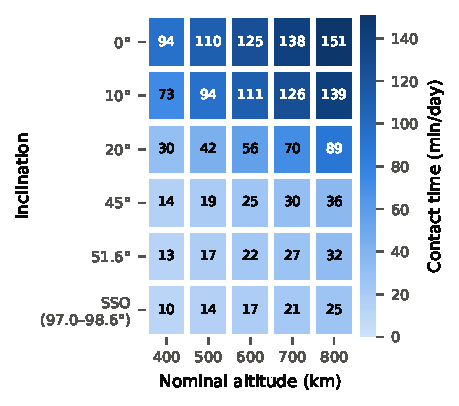
\includegraphics[width=\linewidth]{fig_contact_heatmap.pdf}
\caption{Daily contact time (min/day) for each simulated case, \MaskBase° mask, mean over RAAN. Each cell is one case; nothing is interpolated (SSO: \SSOIncMin°--\SSOIncMax°, set by altitude).}
\label{fig:heat}
\end{minipage}\hfill
\begin{minipage}[b]{0.555\textwidth}\centering
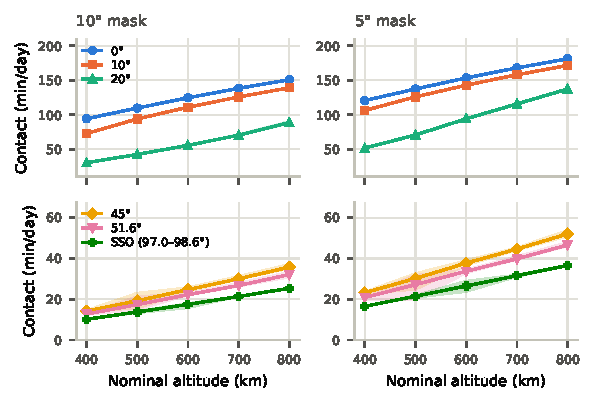
\includegraphics[width=\linewidth]{fig_contact_vs_altitude.pdf}
\caption{Contact time vs nominal altitude for both masks; bottom row (45°, 51.6°, SSO) on its own scale. Lines: mean over RAAN; bands: min--max over the tested starting RAAN (sensitivity to the initial node, not numerical uncertainty).}
\label{fig:alt}
\end{minipage}
\end{figure}

\section{Results}\label{sec:res}
(\lbl{simulated}; \MaskBase° mask, mean over RAAN unless stated.) \emph{Baseline:} 500\,km, 0° gives \BaseN\ passes in the 7-day window, \BasePPD\ passes/day and \BaseCMD\,min/day, consistent with SaRC's figure of about 14; the difference from the \RevsRel\ relative revolutions/day of Section~\ref{sec:interp} is within the counting resolution (Appendix~\ref{app:notes}).

\emph{Per case:} contact time for every altitude and inclination is given in Fig.~\ref{fig:heat}, passes per day in Fig.~\ref{fig:passes} and the gaps between passes in Fig.~\ref{fig:gaps}.

\emph{Trends:} contact time rises with altitude at every inclination and both masks (Fig.~\ref{fig:alt}); at 0° the mean pass lengthens from \MPZeroLo\ to \MPZeroHi\,min. Lowering the mask to \MaskSens° at 500\,km gives about the contact time of 700\,km at \MaskBase° (0°: \MaskZeroB\ vs \MaskZeroC; 45°: \MaskFfB\ vs \MaskFfC\,min/day). \emph{Initial node:} the tested RAAN range can be large (500\,km, 45°: \RaanCMin--\RaanCMax\,min/day; Fig.~\ref{fig:raan}).

\section{Interpretation and implications}\label{sec:interp}
(\lbl{inferred} from the geometry above unless labelled.) A prograde ground track stays between latitudes $\pm i$; NTU is at \StationLat°\,N. For 0° and 10° the track comes within $\lambda$ of NTU on essentially every revolution, so passes per day follow the revolutions relative to the rotating Earth ($\RevsDay-\EarthRevs=\RevsRel$ per day at 500\,km, \lbl{calculated}), and the longer period at higher altitude gives slightly fewer of them. At 10° many passes are off-centre, hence shorter and less contact than at 0°. At 45° and above, only the few revolutions whose track passes near NTU at low latitude give contact (Fig.~\ref{fig:track}), hence the low pass counts and half-day gaps.

\lbl{Observed} at 500\,km (Fig.~\ref{fig:gaps}): at 45°, 51.6° and SSO, contact comes in \WinPerDayMin--\WinPerDayMax\ windows per day of one or two passes (mean \PassPerWinMin--\PassPerWinMax) about one orbit (\GapShortMed\,h) apart, separated by \GapLongMin--\GapLongMax\,h; at 20° the long gaps cluster at \TwGapA\ and \TwGapB\,h.

Altitude acts through three separate effects: $\lambda$ grows, the satellite moves more slowly relative to the rotating Earth, and both make each pass longer, which outweighs the fewer passes. For inclined orbits the track pattern shifts slowly from day to day, so a 7-day window samples few pass geometries, which explains the RAAN sensitivity.

\emph{For contact planning:} a near-equatorial orbit gives frequent contact from NTU, whereas common inclined and SSO orbits should be planned around \HiPLoInt--\HiPHiInt\ passes per day and gaps above \HiGFloor\,h; the site's usable horizon is worth establishing early, as the mask mattered about as much as \MaskAltDiff\,km of altitude in the cases of Section~\ref{sec:res}; and inclined-orbit planning should use the tested range, not a single number. In practice inclination is often set by launch availability (rideshares go mostly to SSO or ISS-like 51.6°; \lbl{context}, not from this analysis), which makes the \HiPLoInt--\HiPHiInt\ passes/day case the likely one.

\section{Limitations and conclusion}\label{sec:lim}
Geometric contact is not usable link time: link budget, antenna pattern and pointing, acquisition, Doppler, scheduling and weather are not modelled, and the \NShort\ passes shorter than 1\,min (\ShortPct\,\% of \NPassesTotal) may carry little data. No drag, which matters most at \HLo\,km. Circular only in the osculating sense (actual mean altitude up to \MaxAltOffset\,km below nominal). One approximately located station, uniform mask (no terrain), J2-only dynamics, no Sun (SSO lighting not represented), \NRaan\ tested RAAN values and one 7-day window; no comparison with measured passes.

From a single station at NTU, inclination decides how often the satellite is in view; altitude and elevation mask then scale the contact time. Next steps: a link budget, a second ground station, a measured site horizon, and drag.

\label{body-end}
\clearpage
\appendix
\renewcommand{\thesection}{\Alph{section}}
\section{Methodological notes}\label{app:notes}
\emph{Counting resolution.} Pass rates are quantised: one pass changes a single run by \ResRunFrac\ = \ResRun\ passes/day and an 8-RAAN mean by \ResMeanFrac\ = \ResMean. At 500\,km, 0°, the \RevsRel\ relative revolutions/day give \WindowRevs\ revolutions in the window, i.e.\ \WindowFloor\ or \WindowCeil\ passes depending on its phase (\lbl{calculated}); the simulated \BaseN\ is one of these, so \BasePPD\ vs \RevsRel\ is within the counting resolution.

\emph{RAAN sampling.} Over the \NInclinedCases\ inclined cases, the mean of the 4-value subset (0/90/180/270°) differs from the 8-value mean by a median of at most \SubsetMedRel\,\% for every metric, and by at most \SubsetMaxRel\,\% in the worst case.

\emph{J2 magnitude.} In the equatorial plane at 500\,km the J2 term is $\tfrac32 J_2(R_\mathrm{eq}/r)^2=\ExAJRatio\times10^{-3}$ of the central term (\ExAJ\ vs \ExAKep\,mm/s$^2$).

\emph{Step size.} For 500\,km, 0°, a rerun with a 30\,s maximum step gave identical pass start and stop times at the report's 1\,ms resolution (durations within \StepDurMicro\,\textmu s).

\section{Supplementary figures}\label{app:figs}
All figures are generated by \texttt{src/make\_figures.py} from the project data; plotted values that the report quotes are checked against the generated numbers.

\begin{center}
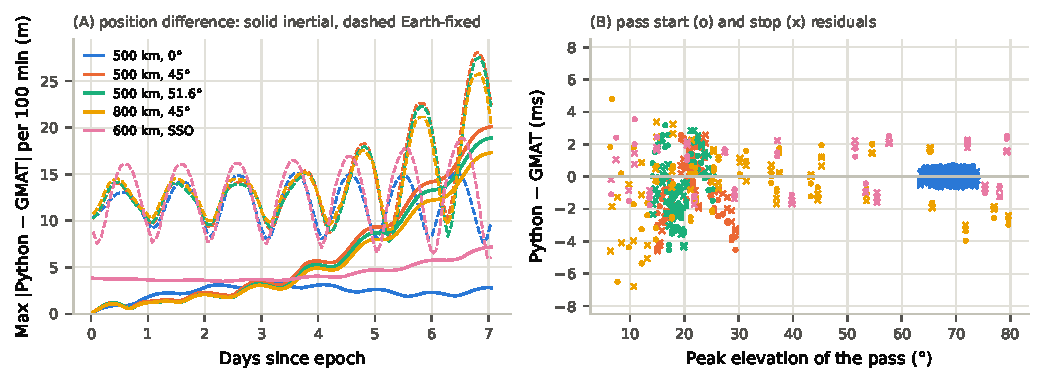
\includegraphics[width=\textwidth]{fig_gmat_python_validation.pdf}
\captionof{figure}{Independent Python vs GMAT, \NXOrbits\ orbits $\times$ \NXMasks\ masks, RAAN 0°. (A) Position difference over the propagation, plotted as its maximum per 100-min interval (an envelope of the per-orbit oscillation); solid: inertial, dashed: Earth-fixed. (B) Pass start (o) and stop (x) timing residuals against the pass's peak elevation (from GMAT's state log: 60\,s samples with a parabolic peak fit); the pre-registered tolerance of \TolEventS\,s is far off scale. \lbl{Observed:} the inertial difference grows over the week for the inclined orbits and stays small for the equatorial one; the Earth-fixed difference is present from the start for every orbit and varies with a period of about one day. In (B) the largest residuals occur on low passes, but peak elevation and orbit are confounded: every equatorial pass is high (peak $\ge$ \EqPeakMin°) and that orbit has the smallest trajectory difference, while the \NIncHigh\ inclined passes that are as high still reach \ResIncHighMaxMs\,ms. \lbl{Hypotheses} (untested): a low pass crosses the mask slowly, so the same position difference shifts the crossing time more; the daily Earth-fixed term comes from the frame conversion (Python applies no polar motion); the inertial growth comes from the different J2-axis treatment.}
\label{fig:val}
\end{center}

\noindent\begin{minipage}[t]{0.49\textwidth}\centering
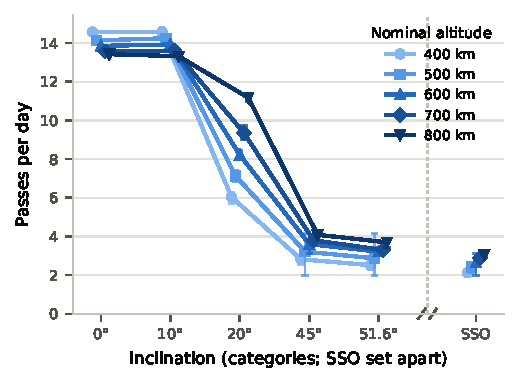
\includegraphics[width=\linewidth]{fig_passes_per_day.pdf}
\captionof{figure}{Passes per day per nominal altitude, \MaskBase° mask, mean over RAAN; bars: min--max over RAAN. Inclinations are categories, with SSO set apart after the break; points are offset slightly per altitude for legibility, and lines join only the fixed inclinations. A pass is a geometric visibility event, not link capacity.}
\label{fig:passes}
\end{minipage}\hfill
\begin{minipage}[t]{0.49\textwidth}\centering
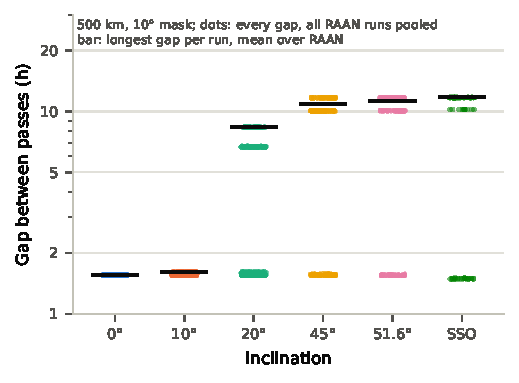
\includegraphics[width=\linewidth]{fig_interpass_gaps.pdf}
\captionof{figure}{Every gap between consecutive passes at 500\,km, \MaskBase° mask, all RAAN runs of a case pooled (log scale; horizontal jitter for legibility only). A gap is the next pass's start minus the previous pass's stop, for passes touching the 7-day window; the time before the first and after the last pass is not counted. Bar: the reported longest gap (per-run maximum, mean over RAAN). The two clusters at 45°--SSO are gaps of about one orbit inside a contact window and the long gaps between windows. Finite-window statistics.}
\label{fig:gaps}
\end{minipage}

\vspace{0.2em}
\noindent\begin{minipage}[t]{0.49\textwidth}\centering
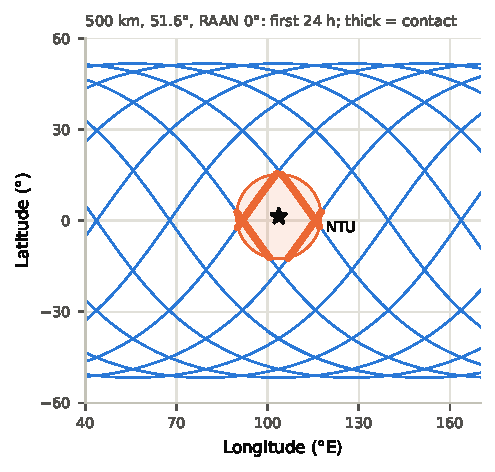
\includegraphics[width=0.88\linewidth]{fig_ground_track_geometry.pdf}
\captionof{figure}{500\,km, 51.6°, RAAN 0°: ground track around NTU over the first 24\,h of the analysis window, from GMAT's state log. Thick: GMAT-reported contact intervals (\MaskBase° mask). Circle: sub-satellite points with NTU elevation $\ge$ \MaskBase° (spherical Earth, at the orbit's mean altitude). Only the few revolutions that pass close to NTU give contact.}
\label{fig:track}
\end{minipage}\hfill
\begin{minipage}[t]{0.49\textwidth}\centering
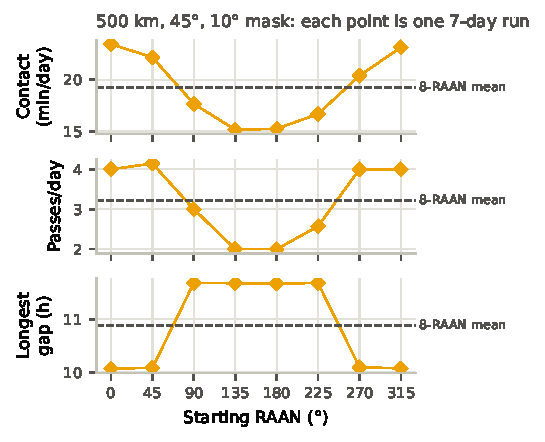
\includegraphics[width=0.88\linewidth]{fig_raan_sensitivity.pdf}
\captionof{figure}{500\,km, 45°, \MaskBase° mask: each point is one 7-day run with a different starting RAAN; dashed: the 8-RAAN mean used in the results. The spread is sensitivity to the initial node position over a finite window, not numerical uncertainty.}
\label{fig:raan}
\end{minipage}

\vspace{-0.6em}
{\footnotesize\raggedright
\begin{thebibliography}{9}\setlength{\itemsep}{0pt}\setlength{\parskip}{0pt}
\bibitem{sarc} Satellite Research Centre, NTU. \emph{Research Capabilities}. \url{https://www.ntu.edu.sg/sarc/research-capabilities} (accessed 2 Oct 2026).
\bibitem{gmat} NASA Goddard Space Flight Center. \emph{General Mission Analysis Tool (GMAT)}, R2026a. \url{https://software.nasa.gov/software/GSC-17177-1}.
\bibitem{vallado} D.\,A. Vallado. \emph{Fundamentals of Astrodynamics and Applications}, 4th ed. Microcosm Press, 2013.
\bibitem{scipy} P. Virtanen et al. SciPy 1.0: fundamental algorithms for scientific computing in Python. \emph{Nature Methods} 17, 261--272, 2020.
\bibitem{skyfield} B. Rhodes. Skyfield: high precision research-grade positions for planets and Earth satellites generator. Astrophysics Source Code Library, ascl:1907.024, 2019.
\end{thebibliography}
}

\end{document}
